% Hazi Feladat / Meresi jegyzokony sablon BME MIT
% Keszult: 2012.13.17
% Leiras: Ebbe a fajlba kerul a lenyegi resz, a szoveg. A legfelsobb szintu felsorolas a section (chapter nem hasznalatos).

\section{A mérés bemutatása}


\section{Otthoni feladat 1}
\subsection{Leírás}
Az LPG tervkészítő runlpg.bat állományának megfelelő átírásával és futtatásával állítson elő olyan terveket (-speed és -quality opcióval is), melyek megoldják a labor weblapján (http://www.mit.bme.hu/oktatas/targyak/vimim223/feladat/3-Tervkeszites) található PDDL források közül legalább… 
\begin{itemize}
\item „Hanoi Tornyai” problémát (3, 5, illetve 7 korong esetén)! 
\item „Műhold” probléma típusos, és numerikus változatát!
\end{itemize}
Hasonlítsa össze, és értelmezze a kapott megoldási terveket (minőség, futási idő, komplexitás szempontjából)!  A kísérletezést a későbbi feladatokkal együtt dokumentálja a labor kapcsán leadandó jegyzőkönyvben (iscreenshot-okkal illusztrálva, igen bő magyarázattal és leírással). 
\subsection{Megoldás}

\begin{tabular}{ l | c | c | r }
	PDDL &  Mode &  Time & Quality \\ \hline
	hanoi3 &  -n 1 &  0.03 &  8 \\
	hanoi3 &   -quality &  0.41  &  7 \\
	hanoi3 &   -speed &  0.05 &  63 \\
	hanoi5 &  -n 1 & 19.28  & 31 \\
	hanoi5 &   -quality & 19.22  & 31 \\
	hanoi5 &   -speed &  19.36 &  31\\
	hanoi7 &  -n 1 & 32.97   & 127 \\
	hanoi7 &   -quality &  37.25 &  127\\
	hanoi7 &   -speed & 37.42  & 127 \\
	műhold(típusos) &  -n 1 & 0.03 & 9 \\
	műhold(típusos) & -quality & 0.05 & 9 \\
	műhold(típusos) & -speed & 0.05 & 10\\
	műhold(numerikus) &  -n 1 & 27.58 & 749.32 \\
	műhold(numerikus) & -quality & 82.83 & 748.03 \\
	műhold(numerikus) & -speed & 27.58 & 748.03\\
\end{tabular}
A feladat követelményének megfelelően futtattam az LPG tervkészítőt. eredményeimet a fenti táblázatban összefoglalva. Megfigyelhetők a következők:
\begin{itemize}
\item A hanoi3 probléma esetében a -quality flag jelentősen megnövelte a futási időt, de sikerült a lépésszámot csökkenteni. Ezzel szemben a -speed flag jelentősen megnövelte a lépésszámot, az általa szolgáltatott terv leginkább egy brute-force megoldásra emlékeztet.
\item  A hanoi5, hanoi7 problémák esetében a különböző flag-ek használata nem hozott jelentős változást; a futási időt inkább a probléma komplexitása határozta meg.
\end{itemize}

\section{Otthoni feladat 2}
\subsection{Leírás}
Ismerkedjen meg alaposan a http://project.mit.bme.hu/vimim223/sites/XY elérésen található web-áruházakkal, majd informálisan (de röviden és tömören) foglalja össze a tapasztalatait:
\begin{itemize}
\item Milyen web-áruházak vannak? 
\item Milyen típusú termékeket árulnak? 
\item Mi jellemzi ezeket a termékeket? 
\item Milyen cselekvési lehetőségek vannak az egyes web-áruházakon belül és kívül? 
\item Milyen egyéb (akár gépi úton letölthető/feldolgozható) információk állnak még rendelkezésre? Például milyen CSV fájlok? 
\end{itemize}
\subsection{Megoldás}
\begin{itemize}
\item a. Milyen web-áruházak vannak? \\
A nekem rendelt weblapon három webáruház érhető el: vörös nagykereskedés, kék webáruház és zöld webshop. 
\item b. Milyen típusú termékeket árulnak? \\
Mindhárom webáruház árul alaplapokat, processzorokat, memóriákat, videokártyákat, merevlemezeket,optikai meghajtókat és monitorokat.
\item c. Mi jellemzi ezeket a termékeket? \\
Ezeket a termékeket jellemzi a gyártó, ár, termékleírás, megbízhatóság, név, termékszám, a termék kategóriája.
\item d. Milyen cselekvési lehetőségek vannak az egyes web-áruházakon belül és kívül? \\
A webáruházakon kívűl megtekinthetjük a vásárolt terméleket, az új egyenlegünket. Letölthetjük a webshopok adatbázisát csv formátumban, továbbá ráléphetünk a webshopokra.
A webshopok oldalán kosárba rakhatunk egy terméket, törülhetjük onnan, elküldhetjük a rendelést.
\item e. Milyen egyéb (akár gépi úton letölthető/feldolgozható) információk állnak még rendelkezésre? Például milyen CSV fájlok? \\
Rendelkezésünkre áll a data.csv ami tartalmazza a következő információkat egy termékről: category;prodname;proddesc;prodinfo;prodprice;prodnum;prodreliability;url
Továbbá letölthető egy compat.csv, ami kompatibilis termékpárokat tartalmaza.
\end{itemize}

\section{Otthoni feladat 3}
\subsection{Leírás}
Indítsunk el Eclipse-ben egy JADE platform-ot, majd futtassuk az PlanExecutorAgent ágenst /jade/src/msclab01/planning\_lab/Planner/testplan.SOL paraméterrel. 
\begin{enumerate}
\item Mit tapasztalunk? Milyen hibákat dob a rendszer, és miért? Hogyan lehet kijavítani? [Tipp: nézzük meg a /jade/src/msclab01/planning\_lab/csv könyvtárban található data.csv minta-termékkatalógusban, illetve az msclab01.planning\_lab.PlanExecutorAgent.PlanExecutorAgent ágens interpretAction metódusában szereplő URL-eket tüzetesebben!!] 
\item Pontosan mi történik az interpretAction metódus végrehajtása során (hogyan interpretálja az ágens a bemenő paraméterként megadott terv lépéseit)? 
\item Futtassa újra az előbbi javítást követően PlanExecutorAgent ágenst, és ellenőrizze az immáron elvileg helyes működést! Megfelelően változott a web-áruházak állapota? Mit történt pontosan?  
\end{enumerate} 
\subsection{Megoldás}
\begin{enumerate}
\item Az ágens forráskódjában az URL-eket kellett kijavítani, aszerint hogy melyik weboldal lett nekem rendelve. Konkrétan az \emph{"http://project.mit.bme.hu/vimim223/sites/00/webshops/shop1/?checkout=1"} kellett átírni \emph{"http://project.mit.bme.hu/vimim223/sites/07/webshops/shop1/?checkout=1"} - re.
\item Az ágens két lépés típust képes végrehajtani: \emph{check-out} és \emph{to-cart}. Mindkét esetben egy url-t térít vissza, ami a konkrét végrehajtandó cselekvést reprezentálja. A \emph{check-out} esetében a csv fájlból kikeresi azt az url ami a lépésben megadott webshophoz tartozik és a rendelés elküldését eredményezi. A \emph{to-cart} lépés feldolgozása abból áll, hogy megkeresi a csv fájban a terméknév alapján azt az url-t ami a terméket hozzáadná a kosárhoz.
\item A fent említett javítás után az ágens sikeresen végrehajtotta a valós cselekvéseket is, vagyis kosárba tette a termékeket és leadta a rendelést.
\end{enumerate} 
\section{Otthoni feladat 4}
\subsection{Leírás}
Töltse le az Ön web-áruházainak teljes kínálatát tartalmazó data.csv termékkatalógust, majd az msclab01.planning\_lab.CSVtable osztály segédlet szerinti felhasználásával (és szükség szerint Microsoft Excel-lel is rásegítve) állítsa elő a letöltött data.csv-nek megfelelő teljes és mintaszerű… a. /jade/src/msclab01/planning\_lab/csv/shopdict.csv és… b. /jade/src/msclab01/planning\_lab/csv/proddict.csv szótárakat! c. Tesztelje az előállt szótárak helyességét a PlanExecutorAgent ágenssel a  3-as feladatban használt testplan.SOL terv megfelelő átírásával! 
\subsection{Megoldás}

A termékszótár előállításához használt CSVtable meghívása:
\begin{lstlisting}[frame=single,float=!ht]
run.bat msclab01.planning_lab.CSVtable data.csv proddict.pddl "2 2" "obj_" ";"
\end{lstlisting}
A shopdict.csv manuálisan lett előállítva, hiszen csak 3 üzlet van
\begin{lstlisting}[frame=single,float=!ht]
PDDL object;Catalog shop
BLUE;blue
GREEN;green
RED;red
\end{lstlisting}
A testplan.SOL megfeleő módosítása után újra futtattam a PlanExecutorAgent-et, ami helyesen lefutott.
\begin{figure}[h]
\begin{center}
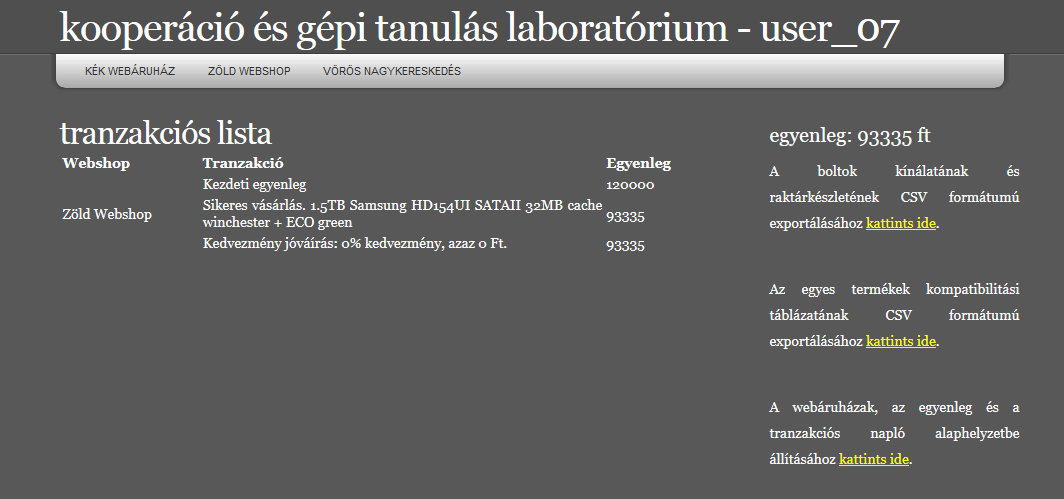
\includegraphics[height=7cm]{figures/web1.png}
\caption{A valós akciók eredménye}
\end{center}
\end{figure}
\begin{figure}[h]
\begin{center}
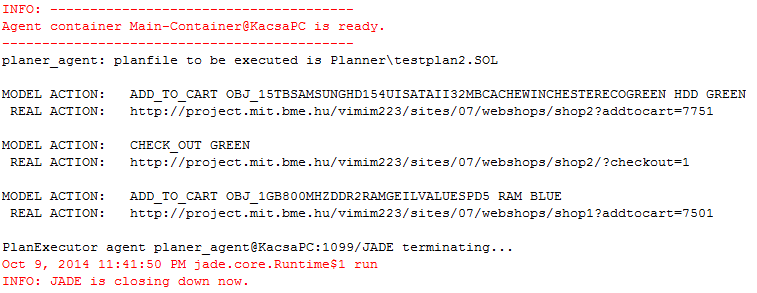
\includegraphics[height=7cm]{figures/dump1.png}
\caption{Az ágens logja}
\end{center}
\end{figure}

\section{Labor feladat 1}
\subsection{Leírás}
Tegyük fel, hogy web-áruházainkban az adott keretek mellett minél olcsóbban szeretnénk hozzájutni egy minél jobb és megbízhatóbb számítógép konfigurációhoz (jelen esetben egy képernyőhöz, egy DVD olvasóhoz, egy HDD-hez, egy alaplaphoz, és egy vele kompatibilis CPU-hoz, videokártyához, és RAM-hoz)! Tegyük fel, hogy a többi szükséges elem már rendelkezésünkre áll (megfelelő billentyűzet, egér, ház, FDD, stb)… 
\begin{itemize}
\item Modellezzük ezt a problémát PDDL nyelven! Hozzunk létre egy absztrakt, formális, PDDL 2.1-es domain- és probléma-leírást a Planner könyvtárban. A probléma- leírásban szereplő objektumokat és kezdeti tényeket az msclab01.planning\_lab.CSVTable osztály segítségével generáljuk. 
\item Oldjuk meg az imént létrehozott problémát LPG-vel, és értelmezzük a kapott megoldási tervet gyakorlati végrehajthatóság szempontjából. 
\item Finomítsuk tovább a PDDL leírást egészen addig, amíg az előálló terv összhangban nem lesz valósággal (azaz addig, amíg a kapott terv lépéseit egyenként végre nem tudjuk hajtani manuálisan, és ennek eredménye valóban nem a legjobb, legolcsóbb, legmegbízhatóbb, kompatibilis számítógép konfiguráció). 
\end{itemize}
\subsection{Megoldás}
\subsubsection{A domain leírás}
\begin{lstlisting}[frame=single,float=!ht]
(define (domain webshop)
	(:requirements :strips :typing :fluent)
	(:types product type shop)
	(:predicates	(compat ?p1 - product ?p2 - product)
						(shopped_from ?s - shop)
						(in_cart ?p - product)
						(in_cart_type ?t - type)
						(prod ?p - product ?t - type ?s - shop)
						(compat_in_cart ?t1 - type ?t2 - type)
						(checked_out ?s - shop)
	)
	(:functions
		(reliability ?p - product)
		(price ?p - product)
		(total_reliability)
		(total_cost)
		(remaining_cash)
	)
\end{lstlisting}
A megoldásomban három típust és ezeken pedig 12 kifejezést. A \emph{product} típus egy terméket képvisel, amiről elmondhatjuk hogy:
\begin{itemize}
\item lehet vele compatibilis termék \emph{compat ?p1 - product ?p2 - product}
\item benne lehet már a kosárban \emph{in\_cart ?p - product}
\item van neki ára \emph{price ?p - product}
\item van neki megbízhatósága \emph{reliability ?p - product}
\end{itemize}
Az \emph{type} jelenti a termék típusát, de ezen kívűl hasznos volt annak a megvalósításában, hogy egy típusú termékből csak egyet vegyünk \emph{in\_cart\_type ?t - type} illetve hogy a termékek kompatibilitás vizsgálatát \emph{compat\_in\_cart ?t1 - type ?t2 - type} véghezvigyük.
A \emph{shop} típus segít abban hogy számon tartsuk melyik üzletből vesszük melyik terméket, illetve hogy melyik üzletekbő kell majd check-outot végrehajtani: \emph{shopped\_from ?s - shop} és \emph{checked\_out ?s - shop}.
Ezenkívül még számon kellett tartanom a teljes árat, maradék pénzt és a teljes megbízhatóságot (\emph{total\_cost}, \emph{remaining\_cash} és \emph{total\_reliability}), amiket a tervkészítő az optimalizálási kritériumként fog használni.
\begin{lstlisting}[frame=single,float=!ht]						
	(:action add_to_cart
		:parameters	(?p - product ?t - type ?s - shop)
		:precondition	(and 	(prod ?p ?t ?s)
					(not ( in_cart_type ?t))
					(>= (remaining_cash) (price ?p))
					(not (checked_out ?s))
							)
		:effect	(and  (in_cart ?p)
				(in_cart_type ?t)
				(increase ( total_cost ) ( price ?p))
				(decrease ( remaining_cash ) ( price ?p))
				(increase (total_reliability) (reliability ?p))
				(shopped_from ?s)
				)
	)
\end{lstlisting}
Az \emph{add\_to\_cart} akció végzi egy termék kiválasztását és a kosárhoz adását. Egy terméket csak akkor választunk ki, ha még nem választottunk egy azonos típusút ki, van elég pénzünk, illetve ha még nem hajtottunk végre check-outot az üzletből. Utóbbi vizsgálata biztosítja hogy csak azután adjuk le a rendelést, miután egy adott üzletnék már nem akarunk több terméket a kosárba tenni. Az akció végrehajtásakor bejelöljük hogy az adott termék és típusa belekerült a kosárba, módosítjuk a teljes árt, teljes megbízhatóságot és a maradék pénzt a termék adatainak megfelelően. Megjegyezzük azt is hogy az adott üzletből vásároltunk, így a végén le is kell adni a rendelést.
\begin{lstlisting}[frame=single,float=!ht]	
	(:action check_compatibility
	   :parameters	(?p1 ?p2 - product ?t1 ?t2 - type ?s1 ?s2 - shop)
	   :precondition	(and 	(prod ?p1 ?t1 ?s1)
								(prod ?p2 ?t2 ?s2)
								(in_cart ?p1)
								(in_cart ?p2)
								( or	(compat ?p1 ?p2)
										(compat ?p2 ?p1))
						)
	  :effect		(and 	(compat_in_cart ?t1 ?t2)
					(compat_in_cart ?t2 ?t1)
					)
	)
\end{lstlisting}
A \emph{check\_compatibility} akció képes a \emph{compat\_in\_cart}-t beállítani, aminek a beállítását majd később a problémaleírásban megadhatunk célként. Csak akkor állítódik be, ha a kosárban levő két termék kompatibilis. Mint látható, maga a \emph{compat\_in\_cart} a termék típusra vonatkozik, így lehetővé válik, hogy a cél definició általánosan csak típusok közötti kompatibilitást követeljen meg.

\begin{lstlisting}[frame=single,float=!ht]		
	(:action check_out
		:parameters	(?s - shop)
		:precondition	(shopped_from ?s)
		:effect		( checked_out ?s)
	)
)
\end{lstlisting}
A \emph{check\_out} egyszerűen a rendelés leadást valósítja meg, jelezvén ezt a \emph{checked\_out ?s} kifejezésben, ami a problémaleírásban a célnál hivatkozható, így biztosítjuk, hogy minden üzletnek leadjuk a rendelést ahonnan terméket tettünk a kosarunkba.
\subsubsection{A probléma leírás}
\begin{lstlisting}[frame=single]	
(define (problem webshop1)
	(:domain webshop)
	(:objects
			cpu hdd videocard display mainboard ram dvd - type
			obj_22SamsungP2270HDLCDmonitorfekete obj_24Samsung2443NWLCDmonitorfekete obj_24LGW2453TQPFLCDmonitorfekete 
			.....
			obj_24Samsung2463UWLCDmonitorfekete obj_26ASUSVW266HLCDmonitorfekete - product
			green red blue - shop)
	(:init
		
		(prod obj_MSIP45C51alaplapLGA775DDR3 mainboard red)
			....
		(prod obj_26ASUSVW266HLCDmonitorfekete display blue)
		
		(= (reliability obj_MSIP45C51alaplapLGA775DDR3) 100)
			....
		(= (reliability obj_26ASUSVW266HLCDmonitorfekete) 100)
		
		(= (price obj_MSIP45C51alaplapLGA775DDR3) 27355)
			....
		(= (price obj_26ASUSVW266HLCDmonitorfekete) 98780)
		
		(compat obj_ASRockM3A790GXH128MalaplapAM3DDR3 obj_AMDPhenomIIX2550dobozosSocketAM3BlackEdition)
			....
		(compat obj_MSIX48CPlatinumalaplapLGA775DDR3 obj_MSIN260GTXLightningBlackEdition1792MBDDR3PCIExpress)
		
		(= (total_cost) 1)
		(= (remaining_cash) 120000)
		(= (total_reliability) 0)
	)
\end{lstlisting}
A probléma leírás a lehetséges \emph{type} egyedek definíciójával kezdődik, majd felsorolja az összes lehetséges terméket, végül magukat az üzleteket.  Ezt követően következik az ismert tények listája, vagyis a termékek jellemzőinek a felsorolása( kategória, üzlet, megbízhatóság, ár, kompatibilitás). Végűl megadtuk a teljes ár, rendelkezésre álló pénz és teljes megbízhatóság kezdeti értékeit.

\begin{lstlisting}[frame=single]	
	(:goal 	(and	(in_cart_type ram)
						(in_cart_type videocard)
						(in_cart_type hdd)
						(in_cart_type mainboard)
						(in_cart_type display)
						(in_cart_type dvd)
						(in_cart_type cpu)
						(compat_in_cart mainboard ram)
						(compat_in_cart mainboard cpu)
						(compat_in_cart mainboard videocard)
						(forall (?s - shop) (and 	(shopped_from ?s)
														(checked_out ?s)
												)
						)
				)
	)
	(:metric maximize (/ (total_reliability)  (total_cost)))
)
\end{lstlisting}
A feladat követelményeinek megfelelően, elvárjuk a tervkészítőtől, hogy egy olyan tervet adjon ahol veszünk minden termék típusból, az alaplap kompatibilis és minden üzletbe leadtuk a rendelést. Azt is megmondjuk, hogy ha lehetséges, optimizálja a tervet, hogy a legolcsóbb legmegbízhatóbb csomagot állítsa össze.

\subsubsection{Eredmény}
\begin{lstlisting}[frame=single,float=!ht]	
; Time 21.23
; Search time 0.39
; Parsing time 20.44
; Mutex time 0.39
; Quality 1.30


Time 21.23

0:   (ADD_TO_CART OBJ_MSIRADEON4830T2D512OC512MBDDR3PCIEXPRESS VIDEOCARD RED) [1]
1:   (ADD_TO_CART OBJ_MSIG31M3LV2ALAPLAPLGA775DDR2 MAINBOARD BLUE) [1]
2:   (CHECK_COMPATIBILITY OBJ_MSIG31M3LV2ALAPLAPLGA775DDR2 OBJ_MSIRADEON4830T2D512OC512MBDDR3PCIEXPRESS MAINBOARD VIDEOCARD BLUE RED) [1]
2:   (ADD_TO_CART OBJ_1GB800MHZDDR2RAMGEILVALUESPD5 RAM BLUE) [1]
3:   (CHECK_COMPATIBILITY OBJ_1GB800MHZDDR2RAMGEILVALUESPD5 OBJ_MSIG31M3LV2ALAPLAPLGA775DDR2 RAM MAINBOARD BLUE BLUE) [1]
3:   (ADD_TO_CART OBJ_22LGW2241SBFLCDMONITORFEKETE DISPLAY BLUE) [1]
4:   (ADD_TO_CART OBJ_INTELCELERON24GHZDUALCORE1MBDOBOZOSSOCKET775E1600 CPU GREEN) [1]
4:   (CHECK_OUT BLUE) [1]
5:   (ADD_TO_CART OBJ_160GBHITACHI7200RPMSATAII8MBCACHEWINCHESTERHDP721016SLA380 HDD GREEN) [1]
5:   (CHECK_COMPATIBILITY OBJ_INTELCELERON24GHZDUALCORE1MBDOBOZOSSOCKET775E1600 OBJ_MSIG31M3LV2ALAPLAPLGA775DDR2 CPU MAINBOARD GREEN BLUE) [1]
6:   (ADD_TO_CART OBJ_LGDH16NS10RBBBSATADVDOLVASOFEKETEOEM DVD RED) [1]
6:   (CHECK_OUT GREEN) [1]
7:   (CHECK_OUT RED) [1]
\end{lstlisting}
Amint látható, a tervkészítő sikeresen összeállított egy olyan lépéssorozatot, ami teljesíti a feladat követelmémyeit. A lépések manuálisan végrehajthatók ebben a sorrendben, jól működnek. Megjegyzendő, hogy a \emph{CHECK\_COMPATIBILITY} lépés úgymond kognitív lépés, tehát nincs valós megfelelője, az eredmény helyesség miatt volt rá szükség.

\section{Labor feladat 2}
\subsection{Leírás}
Indítsunk el Eclipse-ben egy JADE platform-ot, majd… 
\begin{itemize}
\item Frissítsük az 1/c feladatban előállt PDDL leírásnak megfelelően az áruház- és termék-szótárat (illetve szükség szerint esetleg a termékkatalógust is)! 
\item Írjuk át a PlanExecutorAgent ágens interpretAction metódusát úgy, hogy képes legyen feldolgozni az 1/c feladatban előállt megoldási tervet! 
\item Futtassuk a PlanExecutorAgent ágenst az 1/c feladatban előállt megoldási tervvel, és foglaljuk össze, hogy mit tapasztaltunk! Mi kellene, hogy történjen elvben, és mi történik valójában? Helyes ez a működés? 
\item Mi okozhat még problémát elvileg helyes tervek gyakorlati végrehajtása során?
\end{itemize}
\subsection{Megoldás}
A PlanExecutorAgent minimális módosítása után az ágens sikeresen végrehajtotta az előző feladatban elkészített tervet.
\begin{figure}[h]
\begin{center}
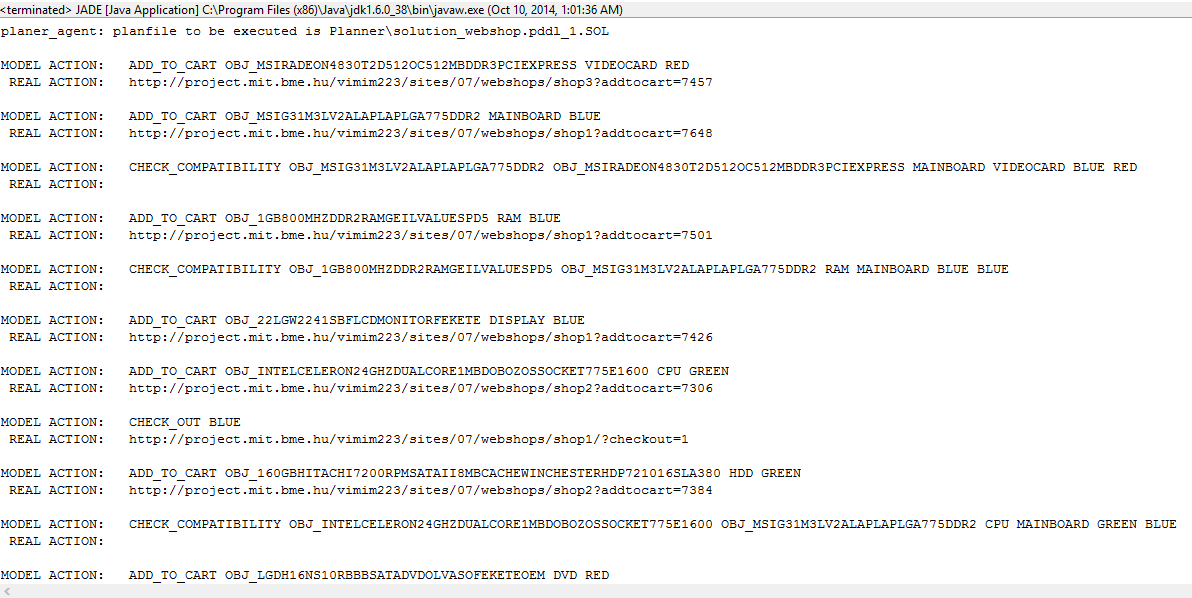
\includegraphics[height=7cm]{figures/dump2.png}
\caption{Az ágens log részlete}
\end{center}
\end{figure}
\begin{figure}[h]
\begin{center}
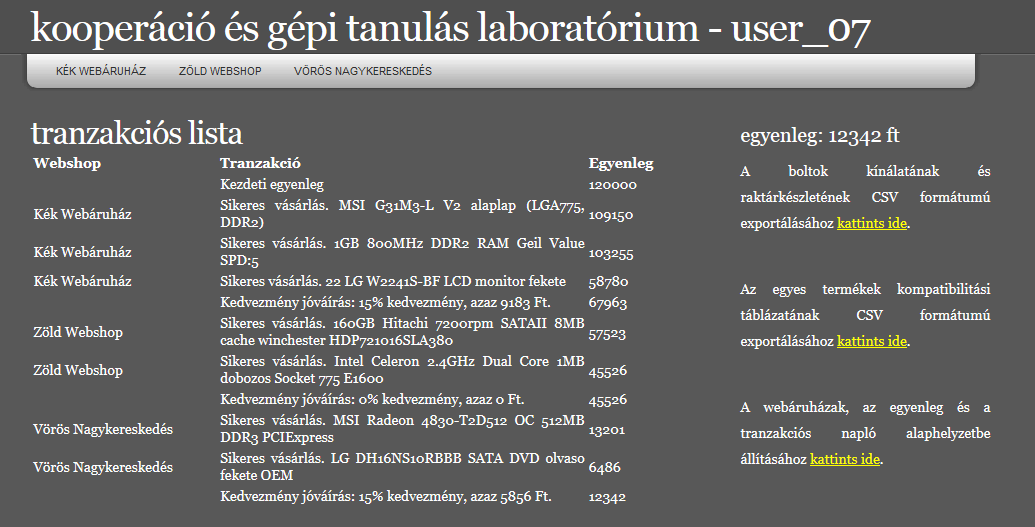
\includegraphics[height=7cm]{figures/web2.png}
\caption{A valós akciók eredménye}
\end{center}
\end{figure}
\section{Összefoglalás}
